% tcm.tex

\documentclass{standalone}

\usepackage{tikz}
\usetikzlibrary{shapes, positioning, arrows.meta, decorations.pathmorphing}

\begin{document}
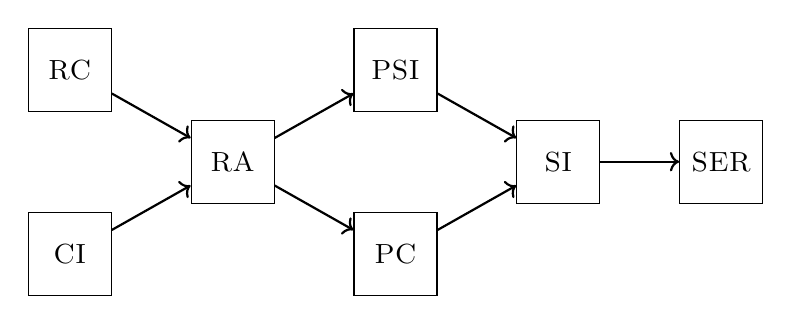
\begin{tikzpicture}[model/.style = {draw, minimum size = 30pt},
  edge/.style = {->, thick},
  node distance = 0.1cm and 1.0cm]

  \node[model] (ra) {\textsc{RA}};
  \node[model, above left = of ra] (rc) {\textsc{RC}};
  \node[model, below left = of ra] (ci) {\textsc{CI}};

  \node[model, above right = of ra] (psi) {\textsc{PSI}};
  \node[model, below right = of ra] (pc) {\textsc{PC}};

  \node[model, below right = of psi] (si) {\textsc{SI}};
  \node[model, right = of si] (ser) {\textsc{SER}};

  \draw[edge] (rc) to (ra);
  \draw[edge] (ci) to (ra);
  \draw[edge] (ra) to (psi);
  \draw[edge] (ra) to (pc);
  \draw[edge] (psi) to (si);
  \draw[edge] (pc) to (si);
  \draw[edge] (si) to (ser);
\end{tikzpicture}
\end{document}